\section{The Projected Grid}
The projected grid is based on a simple concept: in order to achieve an
uniform distribution of details on the image plane, a uniformly spaced grid is
created in post-perspective space and transformed back to world space.
Figure~\ref{fig:projectedgrid} illustrates the difference between a classic
world space approach and the projected grid.
\begin{figure}[h]
\centering
\subbottom[Increase]
{
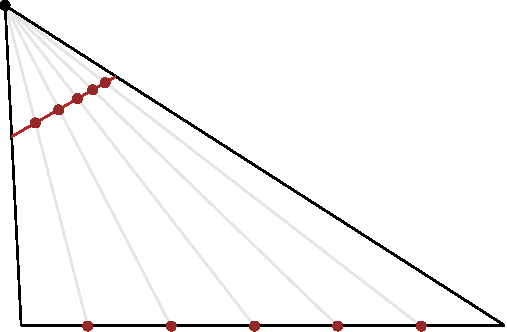
\includegraphics[scale=0.75]{figures/ProjectedGridVsWorldSpace.pdf}
\label{fig:subfigprojgrid1}
}
\subbottom[Increase]
{
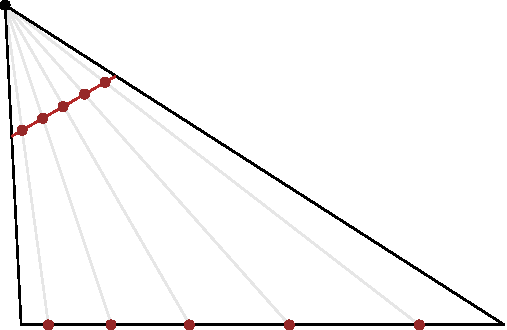
\includegraphics[scale=0.75]{figures/ProjectedGridUniform.pdf}
\label{fig:subfigprojgrid2}
}
\caption[The Projected Grid Concept]{The image on the left shows an uniform
grid in worldspace, its projection onto the image plane is not uniformly
spaced though. The image on the right on the other hand depicts an uniform grid on
the image plane and its associated non-uniform spaced worldspace positions.}
\label{fig:projectedgrid}
\end{figure}

% The algorithm used for the projected grid can be broken down into the following
% steps:
% \begin{itemize}
%  \item create a uniformly spaced grid orthogonal to the viewer using normalised
% device coordinates
%  \item transform the grid to worldspace
%  \item project the grid onto the desired base plane
%  \item apply height displacement
%  \item run the grid through the rendering pipeline as usual
% \end{itemize}

\newcommand{\mvec}[1]{\mathbf{#1}}
\newcommand{\mvecx}[1]{\mathbf{#1}_x}
\newcommand{\mvecy}[1]{\mathbf{#1}_y}
\newcommand{\mvecz}[1]{\mathbf{#1}_z}
\newcommand{\mvecw}[1]{\mathbf{#1}_w}
\newcommand{\mmat}[1]{\mathbf{#1}}
\newcommand{\transpose}[1]{#1^{\mathsf{T}}}
\newcommand{\inverse}[1]{#1^{\mathsf{-1}}}

Let $\mvec{x}$ be a vector representing the three dimensional carthesian
world space coordinate of a vertex, then
\begin{equation}
 \mvec{w} = \transpose{(\mvecx{x}, \mvecy{x}, \mvecz{x}, 1)}
\end{equation}
where $\mvec{w}$ is a homogeneous world space coordinate of $\mvec{x}$.
Let $\mmat{V}$ be the view matrix and $\mmat{P}$ the projection matrix, then
\begin{equation}
\label{eq:ws_to_cs}
 \mvec{c} = \mmat{P} \mmat{V} \mvec{w}
\end{equation}
where $\mvec{c}$ is the \textit{clip space} coordinate of $\mvec{w}$. For $\mvec{c}$ to
be inside the view frustum defined by $\mmat{P}$, $\mvec{c}$ is required to
meet the following condition
\begin{equation}
\label{eq:cs_bounds}
 \mvecx{c}, \mvecy{c}, \mvecz{c} \in \interval{-\mvecw{c}}{\mvecw{c}}
\end{equation}
where $\mvecw{c}$ is the homogeneous component of $\mvec{c}$. Next, clip space
vertex $\mvec{c}$ is transformed by the \textit{perspective division} as follows
\begin{equation}
\label{eq:cs_to_ndc}
 \mvec{n} = \frac{1}{\mvecw{c}}\transpose{(\mvecx{c}, \mvecy{c}, \mvecz{c})}
\end{equation}
where $\mvec{n}$ corresponds to the \textit{normalised device coordinate},
\textit{NDC} in short, of $\mvec{c}$. As one can see, equations~\ref{eq:cs_bounds}
and~\ref{eq:cs_to_ndc} imply
\begin{equation}
\label{eq:ndc_bounds}
 \mvecx{n}, \mvecy{n}, \mvecz{n} \in \interval{-1}{1}
\end{equation}
which defines the space NDC reside in, namely the \textit{canonical view volume},
a three dimensional cube centered at the origin, with a side length equal two.\\


The projected grid, on the other hand, starts inside the canonical view volume
and needs to transform vertices back to world space. Let $\mvec{n}$ be the
normalised device coordinate of a vertex, then
\begin{equation}
\label{eq:ndc_to_cs}
 \mvec{c} = \transpose{(\mvecx{n}, \mvecy{n}, \mvecz{n}, 1)}
\end{equation}
where $\mvec{c}$ is a valid representation of $\mvec{n}$ in clip space. One may choose
a value for $\mvecw{c}$ different from $1$, making it necessary to scale $\mvecx{n}$,
$\mvecy{n}$ and $\mvecz{n}$ accordingly. Again, let $\mmat{V}$ be the view matrix and
$\mmat{P}$ the projection matrix, then
\begin{equation}
\label{eq:cs_to_wsh}
 \mvec{w} = \inverse{(\mmat{P} \mmat{V})} \mvec{c}
\end{equation}
where $\mvec{w}$ is a homogeneous world space coordinate of $\mvec{c}$. Conversion
to three dimensional carthesian world space is accomplished as follows
\begin{equation}
\label{eq:wsh_to_ws}
 \mvec{x} = \frac{1}{\mvecw{w}}\transpose{(\mvecx{w}, \mvecy{w}, \mvecz{w})}
\end{equation}

To simplify matters the grid may be consist of vertices defined by
two-dimensional normalised device coordinates. In order to project the grid
onto a plane a ray has to be setup for every vertex.

postprojection coordinates transformed to worldspace
grid on near and far plane, intersection with the y=0 plane
decouple projector from camera
